\begin{figure*}[t]
    \centering
    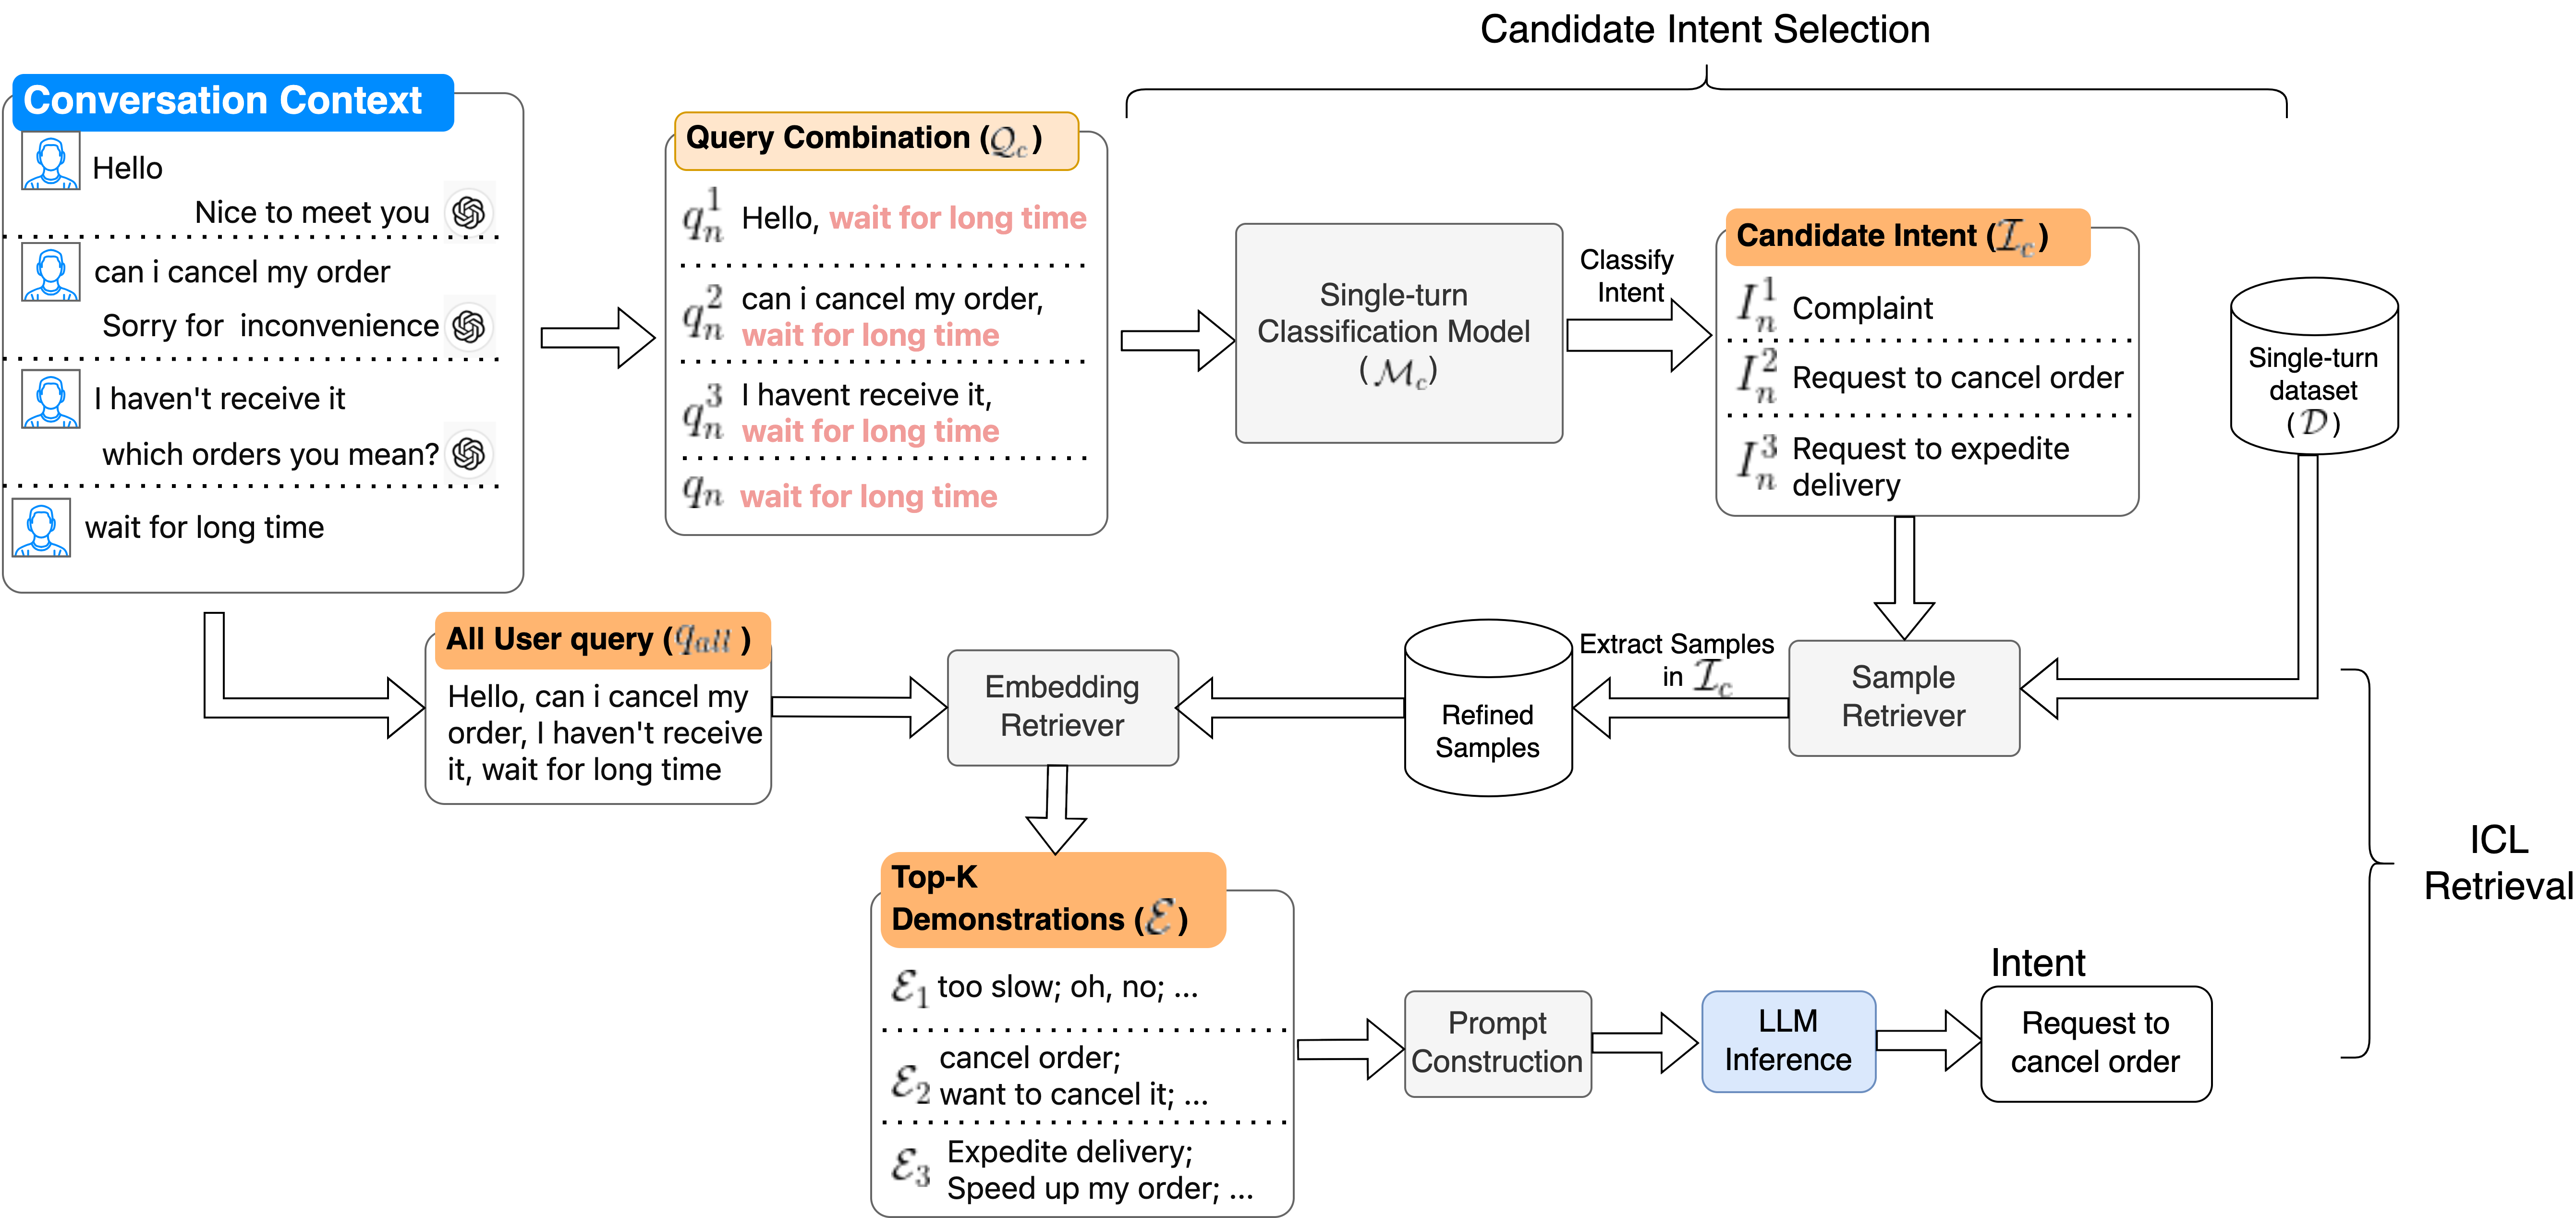
\includegraphics[width=.9\textwidth]{Figures/LLM_in_ICL_way.png}
    \caption{The pipeline of Linguistic-Adaptive Retrieval-Augmentation}
    \label{fig:ICLway}
    \vspace{-0.2cm}
\end{figure*}

\section{LARA: Linguistic-Adaptive Retrieval-Augmentation}



% \subsection{ Supervised Fine-tuning with LLMs }

% % Before delving into LARA, which is the focus of this work, we first consider the supervised finetuning approach. Unlike any other discriminative or regressive methods, we frame this task as a generative one with LLM as the foundation. That is, given the $q_n$ and its context $\mathcal{C}_{\mathcal{Q}\mathcal{I}}$, where the queries and intents are represented in a natural question answering flow of a conversation session $\{q_1, r_1, ..., q_{n-1}, r_{n-1}, q_n\}$, the model is trained to generate the corresponding representative question $r$ of the correct intent $I$ for $q_n$. The complete model input prompt can be found in the appendix. 

% As the Multi-turn Intent Recognition task is formulated as a generative problem, the use of LLMs with suprevised Fine-tuning (SFT) form the foundational approach. Concretely, given the query $q_n$ and its context $\mathcal{C}_{\mathcal{Q}\mathcal{I}}$, where queries and intents follow a natural question-answering flow within a conversation session $\{q_1, r_1, \ldots, q_{n-1}, r_{n-1}, q_n\}$, a model is trained to generate the intent representative query $r$ corresponding to the correct intent $I$ for $q_n$~\footnote{Details on model input prompts are provided in the appendix.}.


% \subsubsection{Compressed Generation} 
% % The representative query $r$ of each intent has on average 12 tokens and are ill-suited to be used as generation labels. The excessive information from the combination of those token count would be wasted considering the number of intents we have, and be unnecessarily complex for model learning. As such, ChatGPT-3.5-turbo is used to compress each $r$ into 2 words in the same language preserving the definition, whereby each intent will be ensured to have different $r_{compressed}$. One of the examples of compressions would be ``How to schedule the date and time of delivery for my order?" $\rightarrow$ ``Order scheduling", where the superfluous information is removed. The compression will start from $r$ with the least words, the logic being that the shorter $r$ will contain less information. If a collision happens after compression, i.e. the new $r_{compressed}$ has been seen before, the ChatGPT-3.5-turbo model will be prompted to compress it again with final word counts increased by 1, until a new $r_{compressed}$ is obtained. After the process, the resulting $r_{compressed}$s have on average 4 tokens. 
% Given that the intent representative query $r$ averages 12 tokens and is thus unsuitable for generation labels, a LLM is employed to condense each $r$ into two words in the same language while preserving the intent's essence, ensuring unique $r_{compressed}$ for each intent. This process begins with the shortest $r$, under the premise that shorter $r$ contains more focused information. In case of duplicate $r_{compressed}$, the model iterates the compression, incrementally increasing word count until uniqueness is achieved, resulting in $r_{compressed}$ averaging four tokens.


% \subsubsection{Cross-Lingual Labels} 

% % For non-English markets, we also tried to compress $r$ into English, keeping $\mathcal{Q}$ in the original language. English is the major language in LLMs pretraining corpus, generating labels in a language they are stronger in could pose lower difficulty.

% For non-English content, $r$ is also compressed into English while maintaining $\mathcal{Q}$ in the original language, leveraging English's prevalence in LLM pretraining corpora to potentially simplify label generation.


The LARA framework shown in Figure \ref{fig:ICLway} addresses the multi-turn intent recognition challenge through zero-shot in-context learning with single-turn demonstrations guided by a crafted instruction prompt. First, a single-turn classification model $\mathcal{M}_c$ is trained on single-turn dataset and used to narrow down the intents to be included in the ICL prompt, which are henceforth referred to as candidate intents. This step is necessary due to the limited LLM context window, and it also helps to filter out extra noise from direct demonstration retrieval. Then, for every candidate intent, in-context demonstrations are selected by retrieving single-turn examples that are semantically similar to the multi-turn test sample. Finally, an instruction prompt for multi-turn classification is formulated by combining the demonstrations and test user queries.


\subsection{Single-turn Classification Model ($\mathcal{M}_c$)}
Before diving into LARA, we must train a single-turn hierarchical text classification model on our single-turn dataset $\mathcal{D}$. The model is an ensemble of a simple label-attention model \cite{zhang2020multi} and a state-of-the-art HTC approach named HiTIN \cite{Zhu2023HiTINHT}. The label-attention model only considers the semantic info of user utterances and label-query attention info, which ignores the hierarchical tree-like structure in our intent system. So, we build model $\mathcal{M}_c$, integrating taxonomic structure via the tree isomorphism network within HiTIN into our label-attention model. More details are provided in Appendix \ref{appendix:a}.

We conduct some experiments on our multilingual dataset. The result in Table \ref{table:htc_improvement} shows that HiTIN alone performs better than the label-attention model, and ensembling the two methods further improves performance on average scores. We will use this model as our baseline and generate candidate intents within LARA.

% The ensemble model forms a strong baseline compared to the flat approach used in the LARA pipeline, which is unaware of the taxonomic hierarchy during the in-context learning process. Hence, the effectiveness of LARA is shown even when compared to a non-basic method.

\begin{table*}[t]
\centering
\scalebox{0.8}{
\begin{tabular}{||l c c c c c c c c c||} 
 \hline
  & BR & ID & MY & PH & SG & TH & TW & VN & avg \\ [0.5ex] 
 \hline\hline
 Traffic weight & 150k & 212k & 27k & 46k & 5k & 36k & 36k & 43k &  \\
 \hline\hline
 Label-attention model & 81.55\% & 87.91\% & 83.73\% & 73.29\% & 83.69\% & 83.11\% & 71.55\% & 74.44\% & 82.30\% \\
 HiTIN & 81.85\% & 89.41\% & 84.57\% & 74.75\% & 84.17\% & 83.67\% & \textbf{75.38}\% & \textbf{75.99}\% & 83.53\% \\
 Ensembled  & \textbf{82.66}\% & \textbf{89.62}\% & \textbf{85.33}\% & \textbf{75.98}\% & \textbf{84.57}\% & \textbf{83.89}\% & 75.19\% & 75.52\% & \textbf{83.94}\% \\[1ex]
 \hline
\end{tabular}}
\caption{Noticeable improvement from adding a state-of-the-art HTC approach.} 
% Ensembling two different methods further improved the performance. The averages are aggregated by traffic weight. }
\vspace{-0.2cm}
\label{table:htc_improvement}
\end{table*}


\subsection{Candidate Intents Selection}
\textbf{Query Combination}: After receiving the context from user side, the last query $q_n$ is first combined with each historical query in conversational context $\mathcal{C}$ to form a query combination set $\mathcal{Q}_c$ = $\{q_n, q^1_n, ..., q^{n-1}_n\}$, where $q^i_n$ means the text concatenation of $q_i$ with $q_n$ using a comma. 

\noindent\textbf{Candidate Intent Recognition}: $\mathcal{M}_c$ predicts few candidate intents $\mathcal{I}_{c}$ from all intents $\mathcal{I}$ on these query combinations $\mathcal{Q}_c$. The $\mathcal{M}_c$ is then used to perform inference on each of the concatenated queries to get a set of candidate intents $\mathcal{I}_{c} = \{I_{q_n}, I_{q^1_n}, ..., I_{q^{n-1}_n}\}$. Finally, we will select the top 3 intents with the highest scores. Note that $\mathcal{I}_{c}$ is a set, so duplicated intents will be removed, and the maximum size of $\mathcal{I}_{c}$ is equal to the number of queries $n$ in a session. 


% \subsection{Candidate Intents Selection}
% In terms of candidate intents selection, not all intents from $\mathcal{I}$ are incorporated into the ICL prompt. Instead, the single-turn classification model $\mathcal{M}_c$ narrows down to a subset of candidate intents $\mathcal{I}_{candidates}$, derived from combining the last query $q_n$ with each historical query in $\mathcal{C}_{\mathcal{Q}}$, forming $\mathcal{Q}_{combinations}$. The model's inference on these combinations yields $\mathcal{I}_{candidates}$, a set removing duplicates with its size, $M$, equating to the session's query count $n$.

% Do note that the combination of the top intents from each $P_l$ might not be a valid intent in the intent taxonomy. Hence, we perform one extra step of beam search decoding on the 3 layers results to get a valid top intent. The selection process is detailed in Appendix \ref{appendix:a.1}.

\subsection{ICL Retrieval}
% For each unique $\mathcal{I}_{candidates}^m$ in $\mathcal{I}_{candidates}$, we retrieve top $K$ $\langle x_i, y_i\rangle$ with $y_i \equiv \mathcal{I}_{candidates}^m$ according to the cosine similarity of $x_i$ to the concatenation of all the queries in conversation $q_{all} = q_1 \circ ... \circ q_{n-1} \circ q_n$. We then have a single-turn task demonstration collection $\mathcal{E} = \{ \{s(x_k^m, y_k^m)\}_{k=1}^K; y^m \equiv \mathcal{I}_{candidates}^m \}_{m=1}^M $ of size $M \times K$, where $s(x_k, y_k)$ is a demonstration written in natural language texts with a sample query $x_k$ and the English hierarchical label name $l$ of its corresponding $y_k$. The retrieval model used is a domain sentence encoder pretrained to be able to retrieve text based on cosine similarity of the embedding vectors it produces. 

% Demonstrations are retrieved from the single-turn dataset for each intent in $\mathcal{I}_{candidates}$. Demonstrations consist of a sequence of annotated examples:
% \begin{displaymath}\{(x_{demo}^1, y_{demo}^1), ..., (x_{demo}^k, y_{demo}^k)\}\end{displaymath}
% where $x_{demo}^j$, $1 \leq j \leq k$ denotes the $j$th single-turn sample query and $y_{demo}^j$ denotes the text representing the label, which in our case is the English hierarchical label name $l$. Demonstrations serve two purposes: (1) provides the LLM with evidence to consult on for decision making, i.e. intents and their example queries content; (2) Specifies an output format that LLM outputs must adhere to, thereby enabling straightforward transformation of the model output in natural language into labels.

However, not all training examples under the candidate's intent $\mathcal{I}_{c}$ will be used in the prompt as demonstrations. Here, the demonstrations refer to a sequence of annotated examples that provide LLM with decision-making evidence and specify an output format for natural language conversion into labels during ICL. Our strategy is to sample training examples that are similar to the test sequence for each candidate intent, a method introduced by \cite{liu2021makes}. In this process, we first concatenate all the queries in the session with a comma to get the test sequence $q_{all}$. Then, $q_{all}$ is mapped to a vector $H_{q}$ using the [CLS] token embedding from a pre-trained sentence encoder, $\Phi_{XLMR}$. After that, we retrieve all the single-turn training samples for each candidate intent from $\mathcal{D}$ using a sample retriever and also encode them using $\Phi_{XLMR}$. With $H_{q}$ as query, we use an embedding retriever to search through the sampled examples to retrieve top $K$ - 1 nearest data examples of each candidate intent based on their cosine similarity to $H_{q}$. Together with the representative query of each candidate intent, the retrieved single-turn samples of all candidate intents form the demonstrations $\mathcal{E}$ for in-context learning. We show the detailed algorithm in \ref{alg:retrieval} below.
 % = \{x_j, y_j\}_{j=1}^{K \times M}



\subsection{Prompt Construction and LLM Inference}
% A multi-turn intent recognition task instruction $\mathcal{T}$ is hand-crafted to guide the model to perform multi-turn intent recognition task by referring to the single-turn demonstrations. The complete input prompt $\mathcal{P} = \{\mathcal{T}, \mathcal{E}, \mathcal{C_{\mathcal{Q}}}, q_n\}$ will consist of the task instruction, single-turn demonstrations, context, and the last query. These components are concatenated together to form a text sequence. One point to note is that, the demonstrations in $\mathcal{E}$ are sorted in ascending order based on their cosine similarity scores to $q_{all}$, regardless of intent. This is due to the sensitivity of LLM ICL to their 

% Taking into account the inference speed requirement of real-time applications, we tried two extra methods to constraint the model to generate only a single-token symbol, unique to each intent. (1) $\mathcal{P}_{symbolic} = \{\mathcal{T}_{symbolic}, \mathcal{E}_{symbolic}, \mathcal{C_{\mathcal{Q}}}, q_n\}$. The original label name $l$ of each $y_j$ in $\mathcal{E}_{symbolic}$ are replaced with single-token symbols, e.g. `A', `B', ..., which bears no meaning to the intents they represented. Explanation will be made in the instruction prompt $\mathcal{T}_{symbolic}$ to link the symbols back to their original intent label $y_j$, and the model is instructed to generated the symbols instead of full label names; (2) $\mathcal{P}_{prepend} = \{\mathcal{T}, \mathcal{E}_{prepend}, \mathcal{C_{\mathcal{Q}}}, q_n\}$. In $\mathcal{E}_{prepend}$, representative symbols for each intent will be prepend to the original label name $l$, such that they are separated by an extra character as boundary, e.g. label ``Food $>$ Cancel order" will be written as ``A $>$ Food $>$ Cancel order" in the prompt. Note that the instruction prompt $\mathcal{T}$ remains the same, the trick is to limit the model generation token count to 1 on API level, such that only the symbols `A', `B', ... will be generated. A map from each symbol to their respective intent will be kept when constructing the prompt. Finally, model outputs are greedily decoded, ensuring efficient and accurate intent recognition. An example of each $\mathcal{P}$ variant can be found in the appendix. 
% To include the conversational context $\mathcal{C}$ into the prompt, we need to concatenate all historical questions into one single text. This is achieved by first adding additional semantic prefixes "[History msg {i}] " to each historical question, where $i \in \{1, ..., n-1\}$, before concatenating them with new line characters. For $\mathcal{E}$, . 
A task instruction $T$ is hand-crafted to guide the model to perform multi-turn intent recognition task by referring to the single-turn demonstrations. The task instruction $T$, combined with demonstrations $\mathcal{E}$, conversational context $\mathcal{C}$, and the query $q_n$, forms the input prompt $\mathcal{P}$ for the LLM. The concatenation of each prompt component into one long text is shown in the appendix \ref{appendix:c}. To accommodate real-time application latency requirements, two additional methods were explored to constrain the model to generate single-token symbols representing intents, detailed as $\mathcal{P}_{symbolic}$ and $\mathcal{P}_{prepend}$, with examples also provided in the appendix. Model outputs are greedily decoded, ensuring efficient and accurate intent recognition.

% \section{Algorithm for ICL Retrieval}
% \label{appendix:c}
% \subsection{Algorithm for Candidate Intent Selection}
% \label{appendix:a.1}

% % TODO: beam search? Wont they question the use of beam size?
% \begin{algorithm}[t]
% \caption{Candidate Intent Selection}\label{alg:candidate_selection}
% \begin{algorithmic}
% \let\oldReturn\Return
% \renewcommand{\Return}{\State\oldReturn}
% \Require {$ \mathcal{Q}_c = \{q_n, q^1_n, ..., q^{n-1}_n\} $}
% \For { each item $q_i$ in $\mathcal{Q}_c$ }
%   \State Get $P_1$, $P_2$, $P_3$ for all three layers from $\mathcal{M}_c(q_i)$
%   \State
%   \State Perform beam search with beam size 5 on $P_1$, $P_2$, $P_3$ to obtain top 1 valid intent $I_i$ in taxonomy
%   \State
% \EndFor
% \Return $ \mathcal{I}_{c} = \{I_n, I^1_n, ..., I^{n-1}_n\} $
% \end{algorithmic}
% \end{algorithm}

\begin{algorithm}[t]
\caption{ICL Demonstrations Retrieval}\label{alg:retrieval}
\begin{algorithmic}
\let\oldReturn\Return
\renewcommand{\Return}{\State\oldReturn}
\Require $\mathcal{I}_c$, $Q$, a positive integer $K$
\State $ \mathcal{I}' = remove\_duplicate(\mathcal{I}_c) $
\State $ q_{all} = text\_concatenate(\mathcal{Q}) $
\State $ H_q = \Phi_{XLMR}(q_{all})^{[CLS]} $
\State
\For { each item $I_i$ in $\mathcal{I}'$ }
  % \State $ X_i = get\_training\_samples\_from\_\mathcal{D}\_for\_intent(I_i) $
  \State /* Sample retriever: Get the single-turn training samples under intent $I_i$ */
  \State $ X_i = sample\_from\_\mathcal{D}\_for\_intent(I_i) $
  \State
  \State /* Embedding retriever: Get embedding for each training sample */
  \State $ H_{X_i} = \{\Phi_{XLMR}(x_j)^{[CLS]}\}_{j=1}^{|X_i|}, x \in X_i $
  \State
  \State /* Calculate text similarity of each training sample with test queries */
  \State $ S_i = \{cosine\_similarity(H_q, h_j)\}_{j=1}^{|H_{X_i}|}$, where $h \in H_{X_i} $
  \State
  \State /* Get top $K$ nearest demonstrations */
  \State $ \mathcal{E}_i \gets $ Top $ (K-1) $ $ x \in X_i$ based on $S_i$
  \State Append $r$ of $I_i$ to $\mathcal{E}_i$ /* add representative query to demonstrations of $I_i$ */
\EndFor
\State
\State $ \mathcal{E} = \{\mathcal{E}_i\}_{i=1}^{|\mathcal{I}'|} $ /* collect demonstrations of all candidate intents */
\State $ S = \{S_i\}_{i=1}^{|\mathcal{I}'|} $
\State Sort $ \mathcal{E} $ by their scores $S$ in ascending order
\State
\Return $ \mathcal{E} $
\end{algorithmic}
\end{algorithm}